% Vandpumpe implementering 

\textbf{Sprinkler} \newline
Sprinkleren kræver et 1/2" gevinds tilslutning. Dette løses vha. en konisk fitting, som har et udvendigt 1/2" gevind i den ene ende og en konisk slangetilslutning i den anden. En alm. husholdningsvandslange sættes på slangetilslutningen med et spændebånd. 

\textbf{Alpha 2 pumpe}  \newline
Alpha 2 pumpens tilslutning er 2" udvendigt gevind. Grundet økonomiske omstændigheder er en hjemmelavet tilslutningsløsning valgt. En drejebænk er benyttet til at dreje 2" forskruninger der ender ud i konisk slangetilslutning. Det drejes i alt 2 stk. Disse slangetilslutninger passer til husholdningsvandslangn og forbindes herved til vandtilførsel og sprinkler.

Figur \ref{lab:fitting_alpha2} viser en af de færdige studser til alpha 2 pumpen. 

\begin{figure}[htb]
\centering
{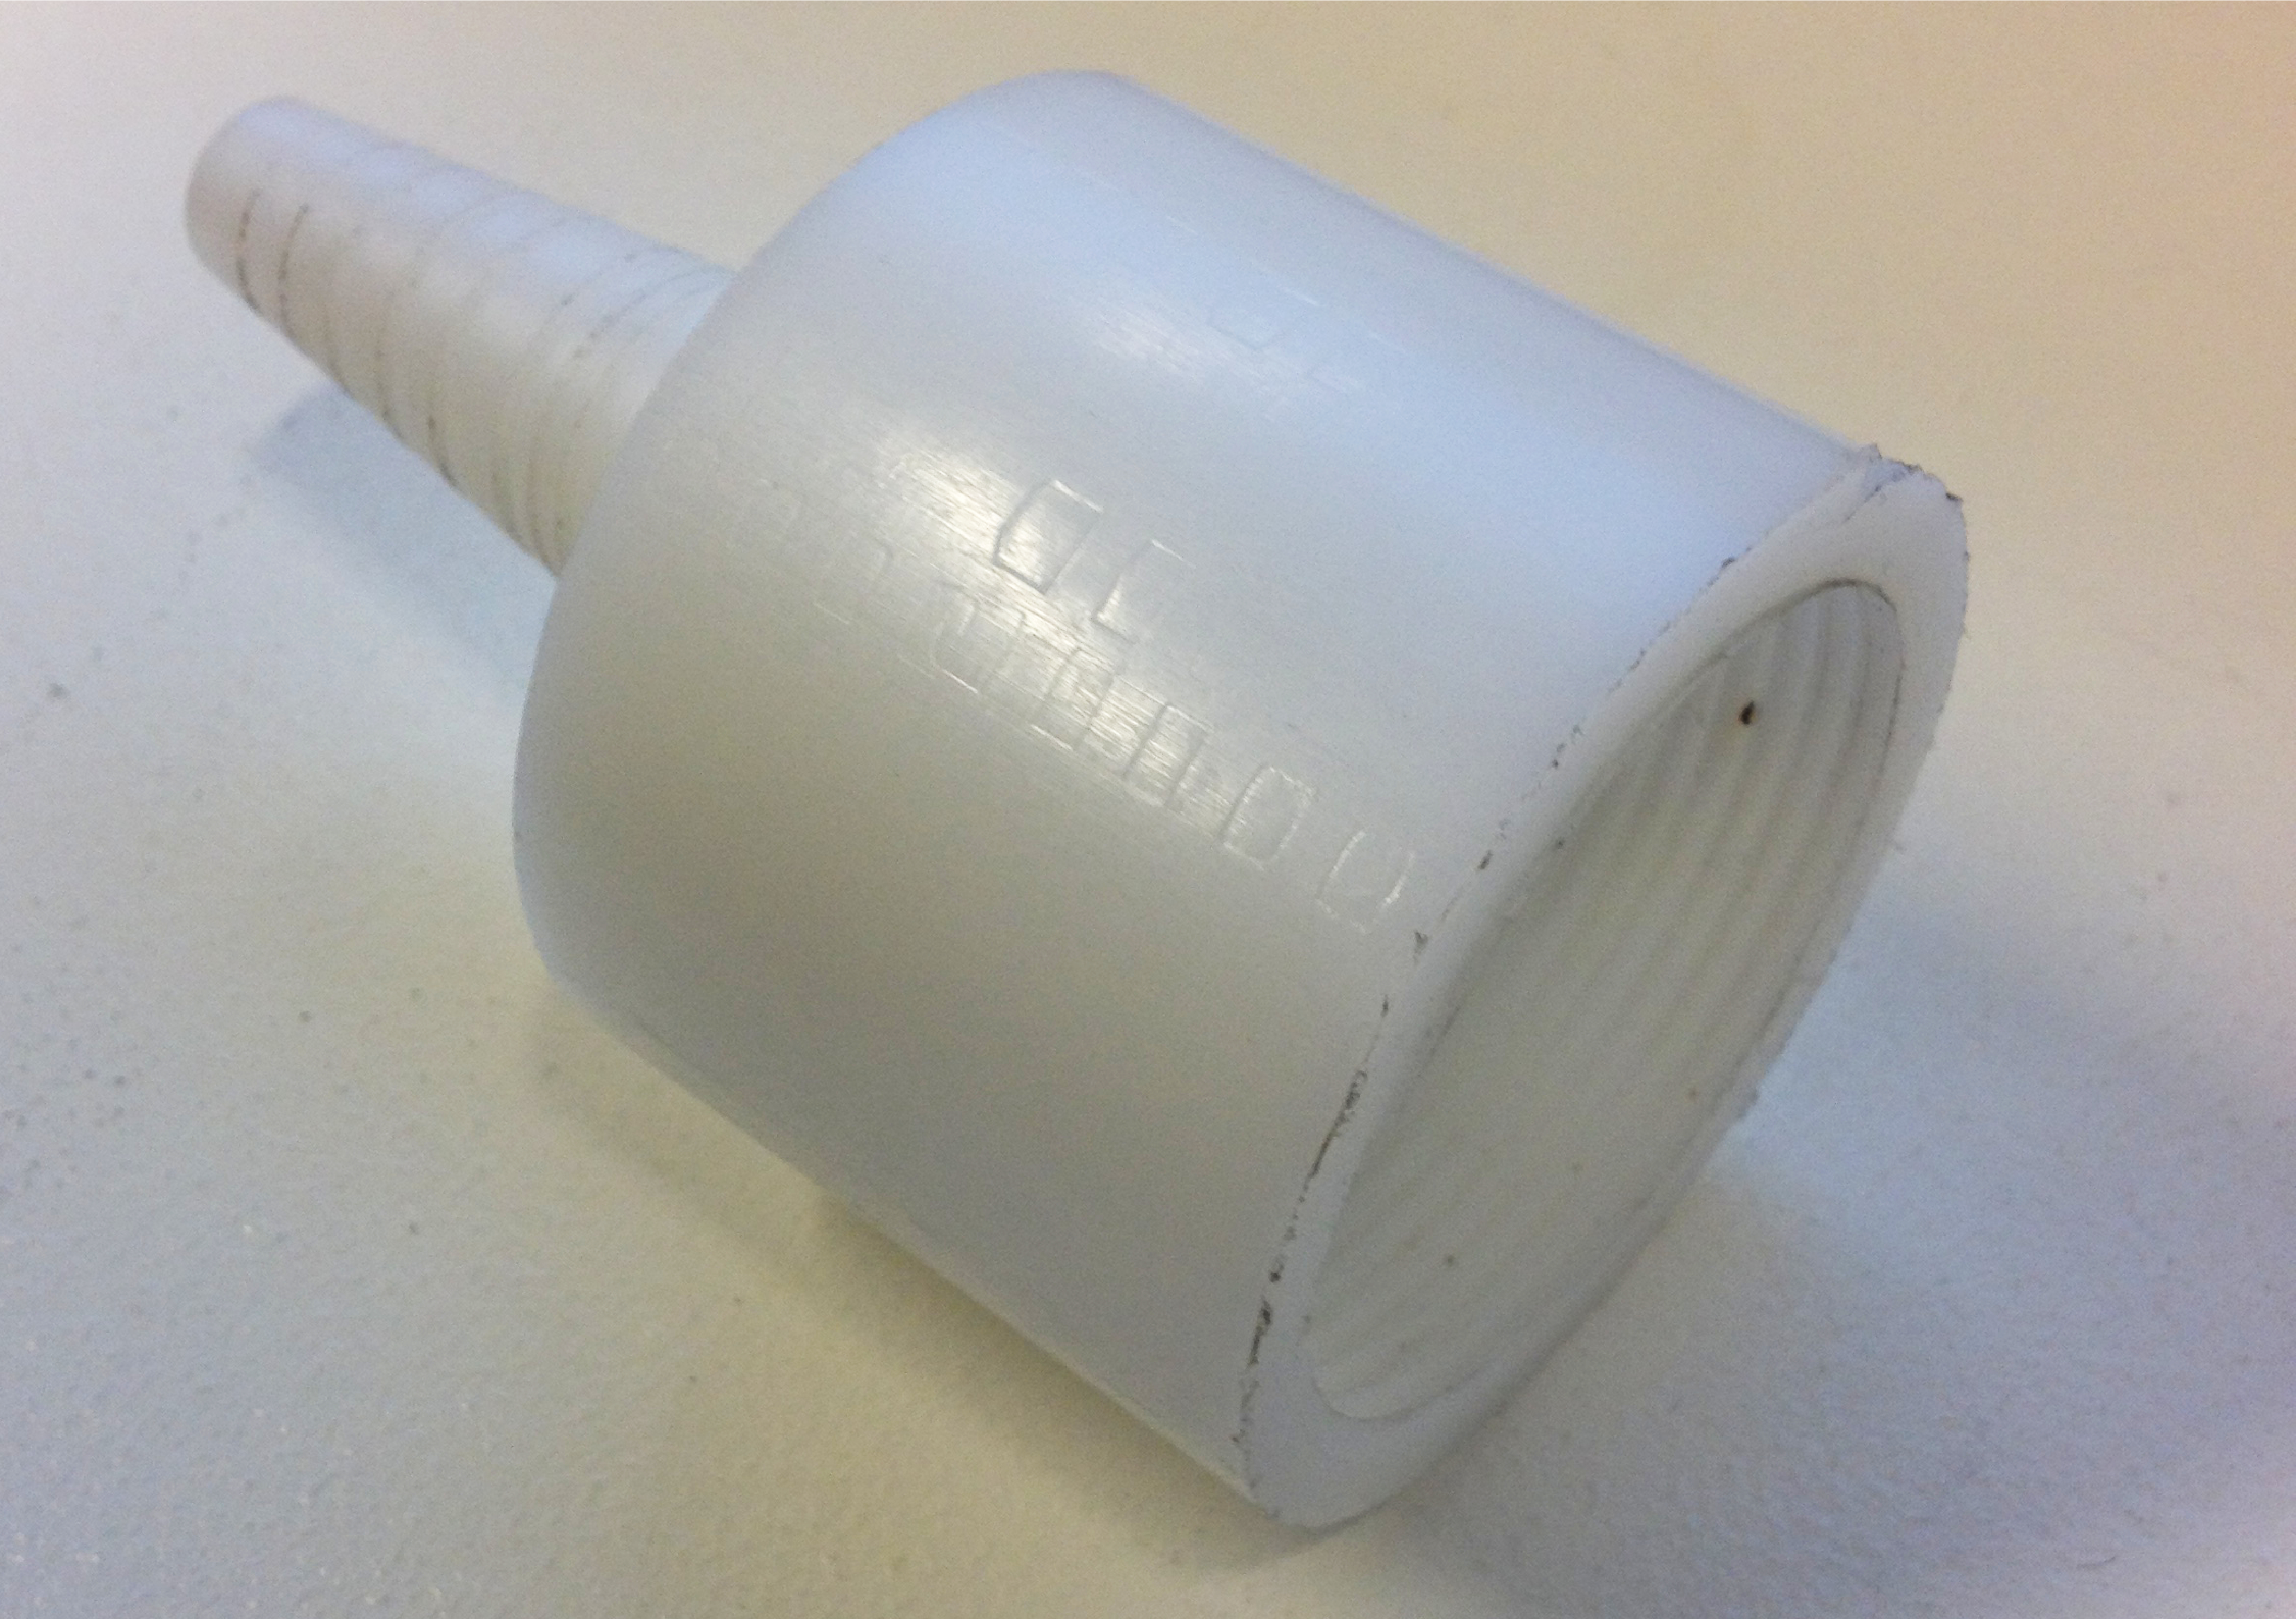
\includegraphics[width=0.60\textwidth]{filer/implementering/studs_alpha2}}
\caption{Studs til Alpha 2 pumpen}
\label{lab:fitting_alpha2}
\end{figure}

